\documentclass[12pt]{report}
\usepackage{xcolor} % for different colour comments
\usepackage{parskip} % Space between each paragraph.
%\usepackage{hardwrap} % for text length of 80 pts
\usepackage[margin=1.2in]{geometry}
\usepackage{hyperref}
\usepackage{../ltx/edcomms}
\usepackage{graphicx}
\usepackage[section]{placeins} % Prevents floats from floating across sections
\usepackage{natbib}%Bibtex
\usepackage{float}

\usepackage{ifthen}
\usepackage{../ltx/edcomms}

%% Comments are enabled and disabled by 'draft' mode. I hacked in my own draft
%% mode (https://en.wikibooks.org/wiki/LaTeX/Macros) because the LaTeX draft
%% mode disables a bunch of things that I don't want it to. I just want it to
%% disable comments. Do not set any of this manually, just use the build script,
%% which builds both draft and final copies. Comments are enabled by default, so
%% if you build manually, you get a draft copy. 
\providecommand\draftmode{true}

\ifthenelse{\equal{\draftmode}{true}}{
\newcommand{\authornote}[3]{\textcolor{#1}{[#3 ---#2]}}
\newcommand{\todo}[1]{\textcolor{red}{[TODO: #1]}}
%\edcommstrue %% Dr. Kahl's comment package. Eventually we should migrate all
             %% comments to this.
}{
\edcommsfalse 
\newcommand{\authornote}[3]{}
\newcommand{\todo}[1]{}
}

% wss = Dr. Smith ; ds = Dr. Szymczak
\newcommand{\wss}[1]{\authornote{magenta}{SS}{#1}}
\newcommand{\ds}[1]{\authornote{blue}{DS}{#1}}



\setlength{\parindent}{15pt} % parskip sets this to 0. 15 is default.
%%%%%%%%%%%%%%%	START OF DOCUMENT %%%%%%%%%%%%%%%%%%%%
\edcommsfalse
\begin{document}

\pagenumbering{roman} %% Roman numerals before actual document starts
\begin{titlepage}\begin{center}
\thispagestyle{empty} %% No page no. on title

\vspace*{1cm}

{\Huge\textbf{Ampersand Event-Condition-Action Rules}}

\vspace{0.5cm}
{\Large Software Requirement Specification 
	
	\edinsert{JG}{Version 1}

\vspace{1.5cm}
Yuriy Toporovskyy,\ Yash Sapra,\ Jaeden Guo}
\vfill

We acknowledge that this document uses material from the Volere Requirements
Specification Template, copyright 1995 - 2012 the Atlantic Systems Guild
Limited.

\vspace{0.8cm}
\end{center}
CS 4ZP6 \\
October 9th, 2015 \\ 
Fall 2015 / Winter 2016 
\end{titlepage}

%% Revision history

\begin{table}[ht!]\begin{center}
\caption{Revision History}  
\begin{tabular}{|l|l|l|}\hline
\textbf{Author} & \textbf{Date} & \textbf{Comment} \\\hline 
Yuriy Toporovskyy & 26 / 09 / 2015 & Initial skeleton version \\\hline
\end{tabular}
\end{center}\end{table}

\tableofcontents
\listoffigures
\listoftables

\newpage
\pagenumbering{arabic} %% Arabic numerals in actual document

%%%%%%%%%%%%%%%%%%%%%%%%%%%%%%%%%%%%
%% Chapter 1: ???                 %%
%%%%%%%%%%%%%%%%%%%%%%%%%%%%%%%%%%%%
\edchange{JG}
{\chapter{Introduction}\label{ch:Intro}}
{\chapter{Project Drivers}\label{ch:Drivers}}

\edchange{JG}
{\section{Project Description}\label{sec:Intro}}
{\section{The Purpose of the Project}\label{sec:Purpose}}
\edcomm{JG}{any comments I made, is a suggestion and its up to you which way 
you prefer to write it. thanks for getting this to us early, I'm sorry we're so 
unorganized}
%% 1a. The User Business or Background of the Project Effort
A large part of designing software systems is requirements engineering. One
of the greatest challenges of requirements engineering is translating from
business requirements to a functional specification. Business requirements are
informal, with the intention of being easily understood by humans; however,
functional specifications are written in formal language to unambiguously capture attributes of the 
information system. Typically, this translation
of business requirements to a formal specification is done by a requirements
engineer, which can be prone to human error.

Ampersand is a tool which aims to address this problem in a different way; by
translating business requirements written in natural language into a formal
specification by means of a ``compilation process'' (\cite{derFun}). 
\edcomm{JG}{Maybe we should cut out how entirely, because there's a design 
specification -- and solely focus on what? thoughts?}%
\edcomm{YT}{The significance of Ampersand has to do with how it solves the
  problem, or how it works. To speak to the purpose of the project means to
  explain why the Ampersand solution is good and why we are spending our time
  making it better. The rubric has a section titled 'General System
  Description', so we need to say something about it}%
%% NB: Put a tex comment at
%% the end of the line after your 'in-line' comments, or latex inserts extra
%% whitespace when rendering with comments off.
Even though the business requirements and formal specification are written in
entirely different languages, the ``compiler guarantees compliance between the
two'' (\cite[2]{derFun}). 

Ampersand also provides engineers with a variety of aids which
help them to design products that fulfill all of the needs of their clients and
the end-users (Figure~\ref{fig:figure1}); including data models, service catalogs and their
specifications. Requirements engineering is perhaps most important in
safety-critical systems; to this end, Ampersand generates modeling aids and
specifications which are provably correct (\cite{derFun}). 

\begin{figure}
  \centering
    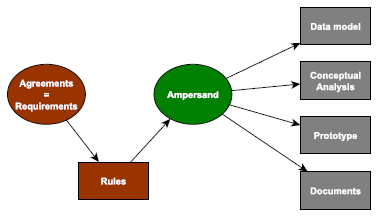
\includegraphics[width=0.7\textwidth]{../figures/ampersand_artifacts}
\caption{Ampersand produces a set of artifacts based on user's requirements.}~\label{fig:figure1}
\end{figure}

%% 1b. Goals of the Project 
Ampersand has proven reliable in practical situations, and there have been
efforts to teach this approach to business analysts. A large portion of the
Ampersand system is already in place; the primary focus of this project is to
augment Ampersand with increased capabilities for automation.

For example, consider a system for ordering products online. Ampersand takes, as
an input, statements of business requirements like
\edcomm{JG}{Good example, could we put something in here about restrictions of 
of the real world?}%
\edcomm{YT}{Business requirements *are* real world requirements. Do you mean something safety-related?
This example isn't the best, I know, but I deliberately chose a simple example}%
\edcomm{YS}{The example is easy to understand. I think we should keep it.} 
\edcomm{YS}{I'm not too sure if the haskell implementation needs to be a part of the introduction.
Rubrics indicate the following critera - - - - %%%%%%%%%%%%%%%%%
 delineate purpose, specify intended audience), system scope, definitions, acronyms,
abbreviations, references, system overview, roadmap of report - - - -
%%%%%%%%%%%%%%%%%%%%%%%
I believe we miss definition of E.F.A and E.C.A since it is being used a lot in the document
}%
\edcomm{YT}{Haskell isn't mentioned at all the intro, ECA is mentioned but is also defined
(it is really quite simple, we don't define it mathematically, just in natural language, so 
it shouldn't be incomprehensible).}%
\begin{quotation}
\noindent{\emph{Every order must have a customer and a list of products; and the total price on
the order must equal the sum of the prices of the products.}}
\end{quotation}
\edcomm{YS}{Attempt at defining ECA}%
\edcomm{YS}{Should we remove some of the haskell code and define the scope of our project in terms of conserving these data rules instead? There's a good chance Dan hasn't read our new problem statement so he doesn't necessarily have a clear idea of Ampersand. Suggestions?}\edcomm{YT}{There is no Haskell code!}\edcomm{YS}{Sorry, i meant the pre-post conditions pairs, I guess we'll let that stay.}%
These are translated into, among other things, formal rules concerning how the
information system must react to changes in its state. Ampersand describes these rules as
a set of Event-Condition-Action Rules (referred to as the E.C.A rules hereafter)
that specify when an event takes place under a given condition, what Action the software must take. 
The information system may contain a function for manipulating orders. (Ampersand can also generate
prototype software models, including functions types like these, from business
requirements - but this is not the topic of our contribution). For example,

\begin{verbatim}
addToOrder : ( o : Ref Order, t : Product )
\end{verbatim}
\noindent{where \verb|Ref x| represents the type of references to values of type
\verb|x|; \verb|Order| and \verb|Product| the types of orders and products, respectively.  }

Ampersand can generate pre- and post-conditions for this function, based on the
business requirements. This constitutes a formal specification of the
information system. For example, the above function may have the following specification:

\begin{verbatim}
{ PRE: o.totalCost = t0 } 
addToOrder(o,t) = ...
{ POST: o.totalCost = t0 + t.cost } 
\end{verbatim}

It is proven \edcomm{YT}{This is 'proven' because someone told me we have a
  proof/presentation of the algorithm, but not its implementation. Can anyone
  find this? We absolutely need a reference to this.} \edcomm{JG}{Can you give 
  me more context as to what is proven? I found an article on ampersand 
  subsets, I pushed it; look for "subsets" by Joosten(both)}%
\edcomm{YT}{There is no file in the repository with the word 'subset' in it?}%
that for the subset of processes which Ampersand can support, there is an
algorithm which will generate the necessary code to satisfy the post-conditions
(ie, formal specifications) of each function. However, Ampersand does not yet
implement this algorithm. Currently, a user of Ampersand must manually indicate
how each violation must be corrected.

In the previous example, the implementation of the
function could be as follows: 

\begin{verbatim}
{ PRE: o.totalCost = t0 } 
addToOrder(o,t) = 
  o.orders.append(t);
  o.totalCost = o.totalCost + t.cost;
{ POST: o.totalCost = t0 + t.cost } 
\end{verbatim}

The first line includes the item in the order, and the second line fixes the
violation of the post-condition which would occur without it. Currently this
second line would have to be hand-written by the programmer, but the
afformentioned \edcomm{YT}{Should have a name to refer to the algorithm
  somehow?} algorithm can derive it from the business rules. The main
contribution of this project will be to implement the algorithm which generates
the code to fix violations.

\section{The Stakeholders}\label{sec:Stakeholders}
%% From the template:
%% For each type of stakeholder, provide the following information:
%% ● Stakeholder identification (some combination of role/job title, person name, and organization name)
%% ● Knowledge that the project needs from that stakeholder
%% ● The degree of involvement necessary for that stakeholder/knowledge combination
%% ● The degree of influence for that stakeholder/knowledge combination
%% ● Agreement on how to address conflicts between stakeholders who have an interest in the same knowledge
%% This doesn't really seem to fit a list format.. And the majority of these things apply
%% mainly to Ampersand - everyone else only uses Ampersand, the developers of Ampersand
%% themselves also need our code to fit into their project, so they have the majority of the say
%% in how things are done. Namely:
%%    A list of the decisions for which the client will be responsible
%% Most 'decisions' will be made by them. 
%% TODO: Write this section. 

\edcomm{YT}{These are the only real stakeholders I can think of...}
\edcomm{JG}{you're right, I can't name names for end users so we might have to cut everything but 
the designers out, or find a way to use the multiple rules the professors have and play in 
dailylife to shovel the other subsections into the first one and strip the subsection titles. I'm 
not sure what to do here  }
\subsection{Ampersand Designers \& Software Engineers}\label{subsec:Ampersand}
Ampersand designers include Dr. Stef Joosten, Dr. Sebastian Joosten and Dr. 
Wolfram Kahl, who in addition to supervising the development of E.F.A are also 
Ampersand contributers. Dr. Stef Joosten is the designer of the Ampersand 
method which have been successfully implemented in various public sectors. The 
interest stemming from these three individuals are not only professional but 
also personal. Ampersand has been nurtured by a great deal of patience and 
dedication. The designers of E.F.A by extension are Ampersand contributors and 
are affected by its outcome, the piece of Ampersand we will build is a 
necessary component required for completion of undergraduate and is designed to 
test the capabilities of an undergraduate team. 
These individuals are the foundation of the belief system by which Ampersand is 
built. The Ampersand model is built on the belief that technology is highly 
incorporated in the use of business and affects the life of every individual. 
It is the belief that information system can and will be designed and built at 
an affordable price and perfectly compliant with the functionalities that users 
desire. This perspective treats information systems as a commodity of the real 
world that can be traded, altered, and used by any individual who is willing to 
learn how to use it.
\subsection{Requirements engineers}\label{subsec:BusReq}
Requirement engineers are responsible of translating business 
requirements into project specifications. Ampersand provides requirement 
engineers with the freedom to explore their creativity rather than be tried 
down by technical minutes. The ability to delegate time consuming tasks such as 
manually checking over technical specifications would increase the efficiency 
of the task at hand as well as decrease the number of hours required for 
completion. An added benefit which engineers receive is the ability to confirm 
that the system they have designed matching the specifications given to them by 
the client. E.F.A provides the ability to ensure no contradictions are found 
within the design by automatically fixing inconsistency that may arise. 
\subsection{Architects \& Functional Specification Designers}
System architects, similar to functional specification designers are 
responsible for various designs which affect procedure and processes in a place 
of business. Ampersand has the ability to confirm that the design provided by 
the Architect matches any building regulations that must be meet. Regardless of 
whether the specification is for safety or aesthetics, the product must meet the 
client's requirements and minimal legal regulations. Ampersand is able to 
compose rules and regulations for data which fully incorporates both without 
contradiction. The addition of E.F.A allows Ampersand to automate correction  
on data which may contradict rules specified for a project. Architects and 
functional specification designers will be able to take advantage of the 
numerous resources Ampersand can provide such as automatic generation of 
databases within prototypes along with tables and relational schema's. 
Furthermore, there is a full range of graphics that stakeholders can choose 
from in order to provide visual display of their design which user may find 
more friendly and easy to understand. 
\subsection{Process Innovators}
Process innovators covers a broad range of individuals that would not commonly 
be considered stakeholders. This broad category includes anyone who provides 
input for business processes which includes both sides of a business agreement, 
in addition to individuals who play a role in seeing the completion of a 
business process. Ampersand allows continuous input as a living system and has 
the ability to reorganize requirements when new constraints are added, and 
E.F.A has the ability to assure the correctness of system information relative 
to the requirements it has been given. With E.F.A's ability to verify 
inconsistencies and automate their correction, changes to design and 
restrictions due to unforeseen circumstances can be added without a system 
overhaul. The efficiency in which Ampersand can provide has the potential to 
dramatically decrease flaws that commonly litter information system.


%%%%%%%%%%%%%%%%%%%%%%%%%%%%%%%%%%%%
%% Chapter 2: Project Constraints %%
%%%%%%%%%%%%%%%%%%%%%%%%%%%%%%%%%%%%
\chapter{Project Constraints}\label{ch:Constraints}
The main constraint of this project is time; this is limited to the 8 month 
period in which we have to build it. It is difficult to perfect an internal 
construction without a large system in such a short amount of time. But time 
restraint is an obstacle which all projects face, because it is not limitless. 
Another major constraint that most project face that this project does not 
require is the financial constraint where projects become difficult to maintain 
and often halt in their progress due to monetary constraints. The lack of 
monetary constraints due to the open source software opens up a broad base of 
opportunities for future improvements and limitless contributions from the 
community.
\section{Mandated Constraints}\label{sec:Constraints}

%%%%
%% 4.1 Solution constraints. 
%% We don't have that many, so 'solution constraints' isn't really appropriate.
\subsection{Project philosophy}

Ampersand is an existing software project with a very sizable code base. The
cost of maintaining poorly-written code can be very high and can outweigh the
benefit of the contribution. In order for our code to eventually be merged into
Ampersand, it must be maintainable: it must be written according to coding
practices of Ampersand; it must be well documented, so it can be easily
understood by other programmers. 

Similarly, our code must not introduce any errors or performance regressions
into Ampersand. Our code must satisfy existing tests and additional tests should
be written for the new algorithm being implemented. Writing maintainable and
well-documented code will help with this goal as well.

These motivations are very important to Ampersand and are considered primary
goals alongside the obvious goal of producing code implementing the desired
feature.

%%3b.
\subsection{Implementation environment}
\subsubsection*{Haskell}
The Ampersand code base is written almost entirely in Haskell. Part of the
prototype software is written in PHP and Javascript %Ref???  
but we likely do not have to interact with this code base. Our code contribution
must be entirely in Haskell.

\subsubsection*{Haskell software}
Ampersand is designed to be used with the Glasgow Haskell Compiler (from here on, GHC) %%REF
and the associated cabal build system. %%Ref
Ampersand also uses many open source Haskell packages, all available on the
Hackage package archive. %% Ref. 
We may not use additional packages. %% Or can we? Maybe if we really needed
                                    %% something, we could ask. But probably not...


\subsubsection*{GitHub}
The Ampersand code base currently lives on GitHub. Our code contributions must
also be on GitHub; this will facilitate easy integration of our code into
Ampersand. This is especially useful if only parts of our code eventually become
integrated into Ampersand - GitHub facilitates this especially. 
\edcomm{YS}{Do we want to tell them that our code might not be integrated in Ampersand?
I think we should abstract this information to make our configuration look more significant.}%

\subsubsection*{Graphviz}
Graphiv is open source graph visualization software, which has the ability to
visually represent information in the form of charts and graphs. It contains
various designs from which the user is able to select. This is used to take
descriptions of graphs in simple text and create diagrams. Ampersand generates
reports about the input system using graphs and charts, so this is one of the
basic components required to run Ampersand.

\subsubsection*{XAMPP}
Ampersand generates prototype websites based on business requirements; to run
these, some web server software is needed. XAMPP stands for cross \big( i.e., X
\big) platform Apache distribution containing MySQL, PHP and Perl. XAMPP \cite{xampp} is the
most convenient way to set up a working database for Ampersand and access .php
pages. 

\edcomm{YT}{Be liberal with what you include in this section, but if it is a
  'technology' then put it in the previous section. Any acronyms, or words that
  the layman probably won't know, need to be here.}%
\section{Naming Conventions and Terminology}\label{sec:Naming} 
\begin{description}
\item[ECA] Stands for Event-Condition Action. The rule structure used for data
  bases and commonly used in market ready business rule engines. ECA rules are
  used in Ampersand to describe how a database should be modified in response to
  a system constraint becoming untrue. Event-Condition Action rules have
  the following structure (\cite[8--9]{RBD}):
\begin{verbatim}
when <some event has happened> 
and if <some condition is fulfilled> 
    do <this activity>
\end{verbatim} %TODO{JG}: bold or italicize words in definitions
\item [EFA] Stands for ``ECA (see above) for Ampersand''.
\item [Functional specification] A \emph{formal} document which details the operation,
  capabilities, and appearance of a software system. 
\item [Requirements engineering] The process of translating business
  requirements into a functional specification. 
\item [Business requirements] Requirements which exist due to some real world constraints;
  ie, financial, logistic, physical or safety constraints. 
\item [Business rules] See \emph{Business Requirements}.
\item [Natural language] Language written in a manner similair to that of human communication; 
  language intended to be interpreted and understood by humans, as opposed to machines. 
\item [ADL] Stands for ``A Description Language'' (\cite[13]{derFun}). From a
  given set of formally defined business requirements, Ampersand generates a
  functional specification consisting of a data model, a service catalog, a
  formal specification of the services, and a function point analysis. An ADL
  script acts as an input for Ampersand. An ADL file consists of a plain ASCII
  text file. 
\item [Ampersand] Ampersand is the name of this project. It is used to refer to
  both the method of generating functional specification from formalized
  business requirements, and the software tool which implements this method.
\edcomm{YS}{ADL is probably not "A data Language".}
\edcomm{YT}{I swear to god I read "A data Language" somewhere... maybe I was
  delirious from lack of sleep... In any case, we should eventually find a
  reference for ``ADL'', whatever it is...}
\edcomm{JG}{this is in Joosten's article "Deriving Functional Specifications from Business 
Requirements with Ampersand", ADL is a tool that accompanies Ampersand (which is a method); ADL 
generates a functional specification consisting of a data model, service catalogue, a formal 
specification of the services, and a function point analysis
	
	It (ADL) translates business rules  back into the natural language, and provides feed back to 
	the requirments engineer for validating his work. (Also becareful with how you use the word 
	validation vs. verification, these terms are distinguished in Rule based design and we dont 
	want to contradict ourselves/our supervisors by using them interchangably)
	
	ADL translates the entire set of requirements to design artifacts that are needed in subsequent 
	software design processes (p.2)
	
	They also specify the difference between requiement and specification: where specification is 
	used to prescribe properties of a system to be built; and requirement describes an explicit or 
	implicit need need of users}
\edcomm{YT}{Stef's article describes ADL as 'an accompanying tool' but also as
  the 'language which is input to Ampersand'. This is confusing and I feel like
  the former definition is not that useful so I decided to omit it. Just refer
  to 'Ampersand' as both the tool which is written in Haskell and this method of
  generating functional consraints from business requirements. To this end, I
  added a definiton of 'Ampersand'. But thanks for the reference to 'A
  description language'}
\end{description}

%TODO{JG}: add Expression as a data type? Find a better way of describing 
%Expression without implementation details

%% This section is strange and we may have to replace it with something else...
\section{Relevant Facts and Assumptions}\label{sec:Assumptions}

%%%%%%%%%%%%%%%%%%%%%%%%%%%%%%%%%%%%%%%%%%
%% Chapter 3 -- Functional requirements %%
%%%%%%%%%%%%%%%%%%%%%%%%%%%%%%%%%%%%%%%%%%
\chapter{Functional Requirements}\label{ch:Functional}
%% This section is probably a good place to give a description of ampersand. 
\section{The Scope of the Work}\label{sec:ScopeOfWork}

\begin{figure}[!htb]
\begin{center}
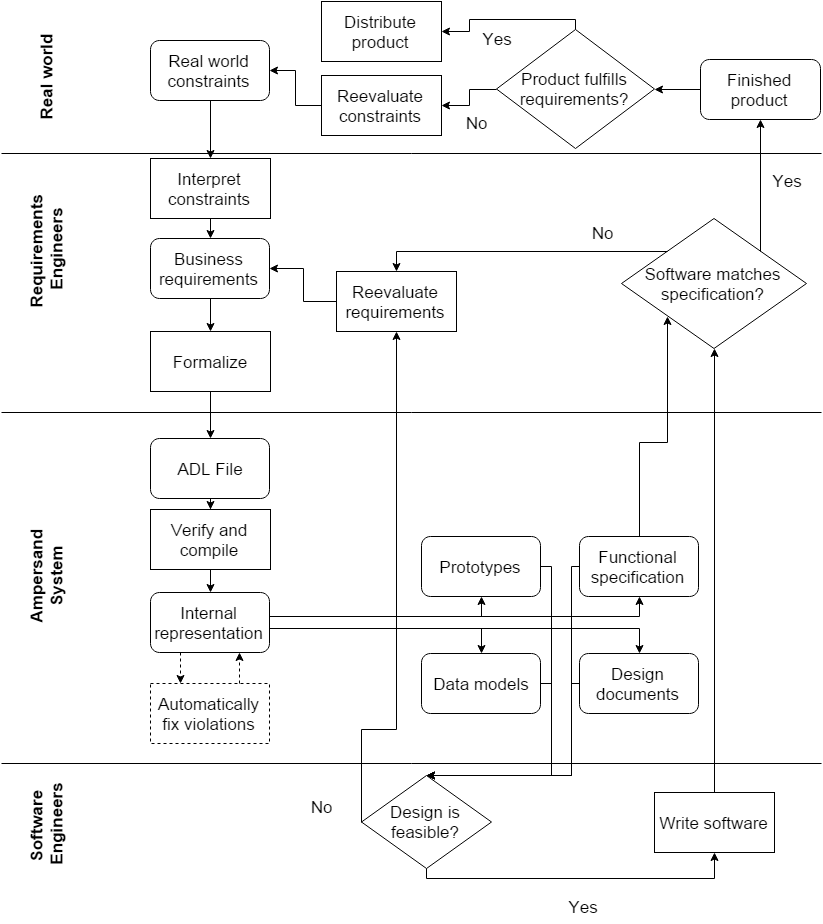
\includegraphics[width=0.6\textwidth]{../figures/business_process}
\caption{The role of Ampersand in the software design cycle}~\label{fig:BusinessProcess}
\end{center}
\end{figure}

Figure \ref{fig:BusinessProcess} is a simplified view of the software design
cycle, intended to highlight the role of Ampersand in this cycle. This view
omits many of the uses of the design artifcats generated by Ampersand; instead
it focuses mainly on the primary purpose, which is to help create a finished
software system. The contribution of this project is denoted with dashed lines.

\section{Business Data Model and Data Dictionary}\label{sec:DataModel}

\section{The Scope of the Product}\label{sec:ScopeOfProduct}
\section{Functional Requirements}\label{sec:Functional}
\subsection{Input}
\subsection{Correct Translation of Input}
\subsection{Output}

\chapter{Non-functional Requirements}\label{ch:NonFunc}
Non-functional requirements are fundamental to the success of any product on the market. This type 
of requirement is especially important to this project as it heavily relates the needs of the 
clients to the changes that need to be made to the final product before it is ready for the public. 
The human element guides the principals introduced in non-functional requirements, and for this 
project, it is motivated by a simple perspective. Tools should make a user’s job easier to do, and 
for that to happen the user must be able to under how to use it. 
\edcomm{JG}{How do I pull the tree up to the first page of non-functional?? *facepalm* 
\vspace{-finity} doesnt work}
\edcomm{YT}{LaTeX floats have 'position modifiers'. Generally you should use
  !htb, this works in over 99 percent of case in my experience. Full details of floats and their positioning here:
  https://en.wikibooks.org/wiki/LaTeX/Floats,_Figures_and_Captions }
\begin{figure}[!htb]
	\centering
	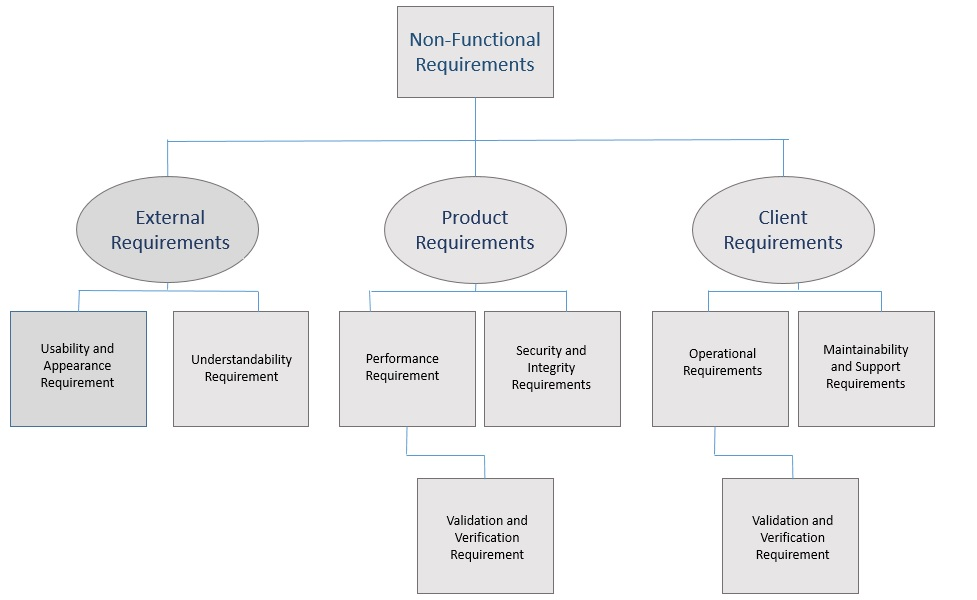
\includegraphics[width=0.8\textwidth]{../figures/NONFUNCTIONAL}
	\caption{Tree of non-functional requirements as it relates to E.F.A.}~\label{fig:figure2}
\end{figure}
\section{Look and Feel Requirements}\label{sec:LookAndFeel} 
Non-functional requirements are fundamental to the success of any product on the market. This type 
of requirement is especially important to this project as it heavily relates the needs of the 
clients to the changes that need to be made to the final product before it is ready for the public. 
The human element guides the principals introduced in non-functional requirements, and for this 
project, it is motivated by a simple perspective. Tools should make a user’s job easier to do, and 
for that to happen the user must be able to under how to use it.  



\section{Usability and Humanity Requirements}\label{sec:Usability}
E.F.A. is built as an internal structure of Ampersand and does not have a graphical interface for 
users. Ampersand uses the command prompt to compile user prototypes which includes various 
graphical representations and webpages. It is very unlikely that users will be able to distinguish 
E.F.A. from Ampersand, it would be similar to someone attempting to distinguish a person’s hand as 
a separate entity from that person. E.F.A. may not look very personable, or user friendly, but it 
will hopefully relieve some frustration and make the user feel more at ease with their design 
because if things do not line up, there is something that can automatically fix it for them. It 
would be another thing users would not have to worry about when designing a new system, this 
feeling of ease could extend to smooth the interactions between the designer and the client as it 
goes through various cycles of overhaul. The user will be notified of any changes that have been 
made to their design and from there Ampersand provides options of how much of the changes the user 
would like to keep, fix themselves, or add to a repository of changes to keep in mind for future 
instances. Thus E.F.A. can return corrections according to what the user specifies.

This product shall be used by any individual who is willing to dedicate the time to learning the 
basics of the Ampersand model and wishes to design an information system. The time it take to learn 
Ampersand is truly up to the user, a normal individual may take anywhere from a week to a month. 
While an engineer who has a strong background in mathematical logic or minor experience in 
programming will be able to use Ampersand efficiently within a week. The most pronounced problem 
concerning Ampersand’s usability is that it’s limited to two languages: English and Dutch. Those 
who are not fluent in neither of these languages will have great difficulty learning the Ampersand 
system.

However, since Ampersand is a successor of CC, \cite[p.10]{RBD}
and similarly it could be used to create consensus between groups of stakeholders with strong 
diverging opinions on the same matter. Once the prototype is generated, it can be presented to 
different individuals who may wish to conduct their own investigation concerning the best course of 
action. After the creation of the prototype, common users are able to manipulate various aspects of 
a project due to an autofill feature. 
\begin{figure}
	\centering
	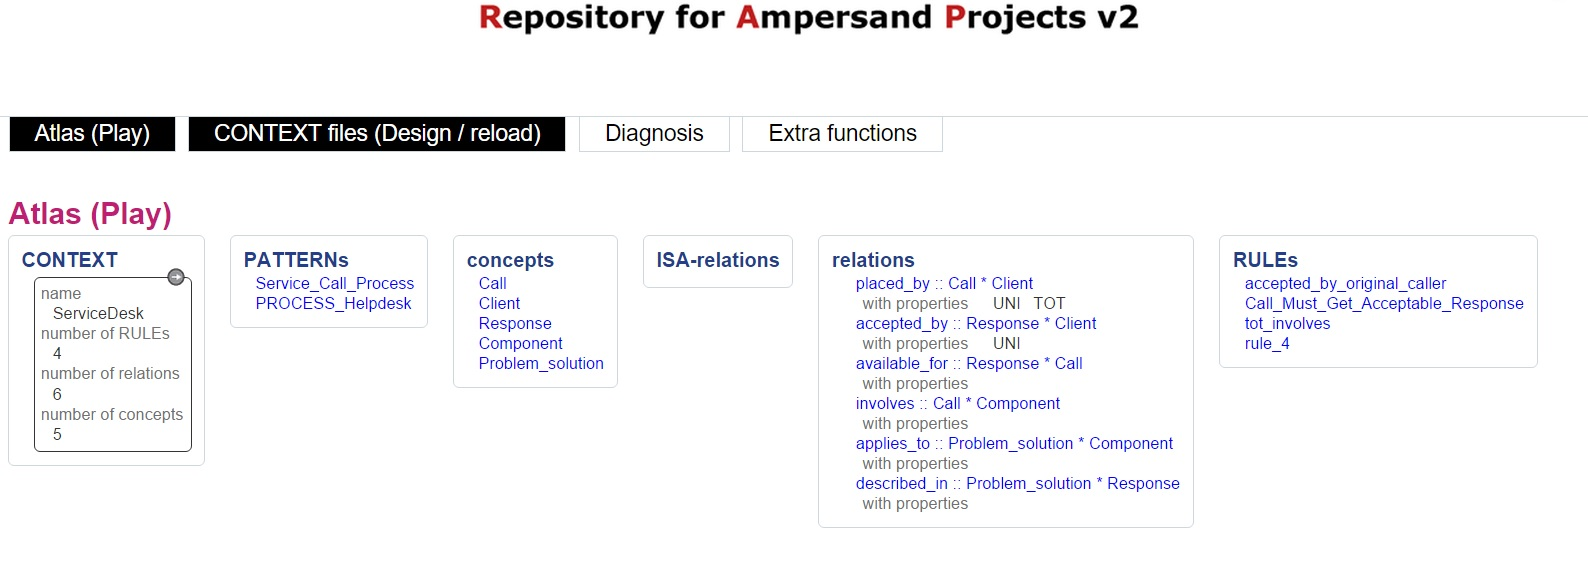
\includegraphics[width=1.0\textwidth]{../figures/Ampersandmodel}
	\caption{An example of what Ampersand users see when they compile a prototype, each tab and 
	figure they have created can be modified.}~\label{fig:figure3}
\end{figure}

\section{Understandability}
What E.F.A. does is simple to understand, it fixes logical inconsistencies with minimal if any 
input from the user. It looks for contradictions and violations, an overly simplistic but accurate 
example would be: a chair is red, a chair is blue, and there is only one chair. That chair cannot 
be blue and red simultaneously, to fix the problem either another chair is added or one of the 
colour conditions is eliminated. What is eliminated may be based on what is more important for the 
system and the user. In the previous example, if it is most important that there is only one chair, 
then one of the colours statements is erased. Otherwise, E.F.A. could add a new chair, now ever if 
adding a new chair decreases the efficiency of the system because it must keep track of two chairs 
now. It may pick a chair colour depending on another criteria that is not directly part of this 
problem. Such as if most individuals who may use the chair prefer it to be red rather than blue. 
That may be an external condition that Ampersand has been programmed to keep in mind. 
\begin{figure}
	\centering
	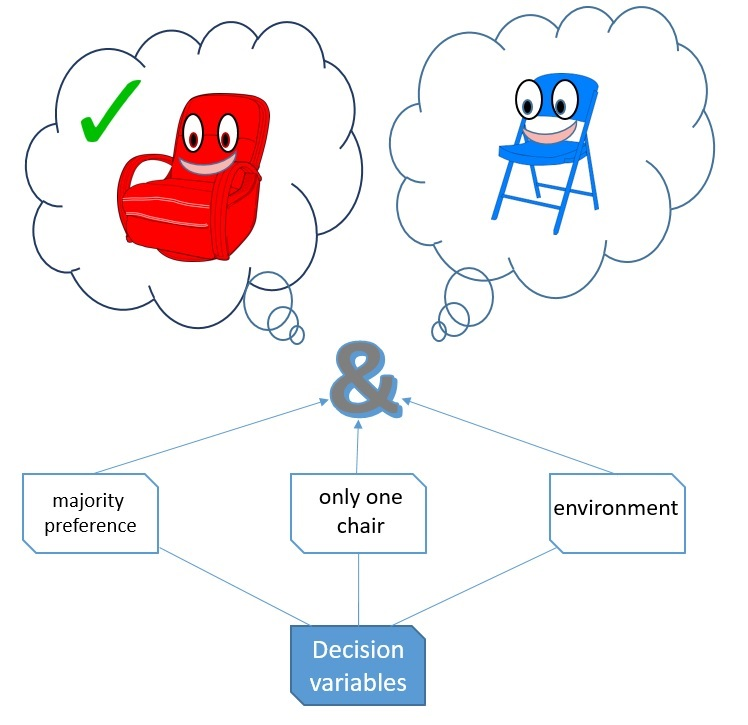
\includegraphics[width=0.5\textwidth]{../figures/blueorredchair}
	\caption{Simplistic diagram of decision making process, for full example of decision making 
	process see. Figure 5.}~\label{fig:figure4}
\end{figure}

\section{Performance Requirements}\label{sec:Performance}
Ampersand can efficiently process a large amount of information in a short amount of time, the 
process that E.F.A. requires will be added onto Ampersand’s process time. The duration of time it 
would take to verify data inconsistencies would depend on the complexity of the system design and 
the number of corrections it may take to update the system to a valid prototype according to 
specification. The current upper bound is expected at 120 seconds, or 2 minutes, the correction 
process is terminated if exceeds beyond this threshold for simple Ampersand models. The prototypes 
termed ‘simple models’ are tasks that can be accomplished by an individual within a short amount of 
time, such as selecting the best actor/actress to play lead according to experience and audience 
appeal. Simple models are able to take into consideration not only the task at hand but the context 
and environment to which the task must be completed in. Performance is measured on speed, but also 
on validation of limitations set forth by the user; it will not matter how quickly E.F.A. can do 
something if it does it incorrectly and creates more work for the user. Currently, the 
quantification of the desired accuracy of the results produced is unknown, as E.F.A. is in its 
initial stages. Furthermore, the allowable time between failures is unknown and untested.

E.F.A. can be a great tool, but in case of failure, in the unlikely event that errors are 
propagated through the system and no one through any cycle of development catch it. If the designer 
puts full faith in E.F.A. it could be catastrophic, especially if mistakes are not caught and 
products proceed into the production stage. However, Ampersand possess an internal structure to 
detect inconsistencies and allows for manual correction. E.F.A. although important is not the last 
line of defense, this secondary system greatly minimizes the chances of complete failure. The 
likely if E.F.A. completely fails, is that the secondary system detects errors and compels users to 
manually correct data (\cite[153]{RBD}). 

\begin{figure}
	\centering
	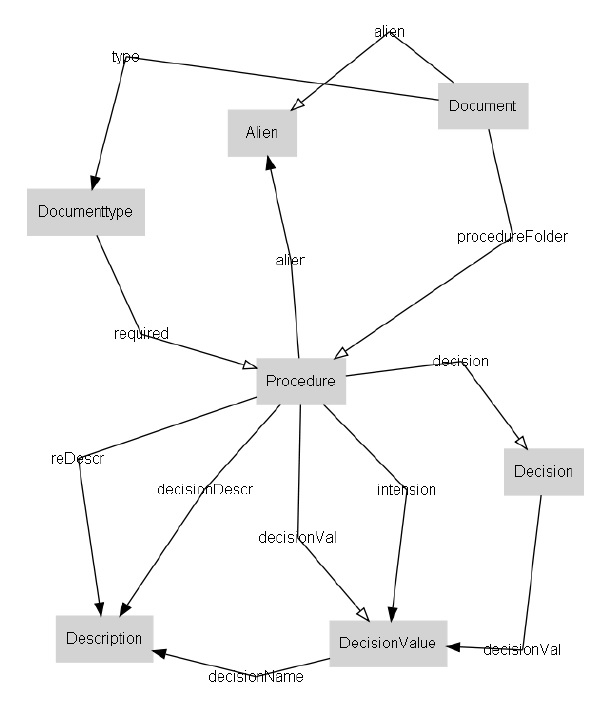
\includegraphics[width=0.5\textwidth]{../figures/Ampersanddecision}
	\caption{This is an example of Ampersand's complete decision process. Source : Rule Based 
	Design}~\label{fig:figure5}
\end{figure}
\section{Operational and Environmental Requirements}\label{sec:Operational}
It is not feasible to predict an accurate workload capacity for E.F.A. for its state, however, 
E.F.A. is made to handle Ampersand loads interactively and is not designed to accumulate stored 
data but rather return the user a modified version of the input they submitted. E.F.A. is meant to 
operate locally within Ampersand, there no limit to the number of users that can use this product. 
Extensive maintenance is not required, although minor adjustments and additions may be necessary 
for further improvement. As Ampersand grows in popularity, it will not be necessary for E.F.A. to 
grow in proportion to Ampersand to remain useful. Due to this it is difficult to determine the 
longevity of this project, as it could remain until the client determines the current model is no 
longer useful. 

Any system that is capable of running Ampersand is automatically compatible with E.F.A., currently 
those system are limited to Windows OS 7 and up. There are very few physical conditions required to 
maintain E.F.A. and they are the basic conditions required to keep most computer system running. 
This includes minimal moisture, and temperatures no lower than 35 (degree farenheight) or 1.7 
(degree celcius) %TODO{JG}:insert appropriate symbols for temperature.
as computer hardware of 
%change by flexing \edcomm{JG}{Is this common knowledge or does this need a citation?} and 
%temperatures preferably no higher than 90 (degree Farenheight) or 32.2 (degree celcius)

\section{Maintainability and Support Requirements}\label{sec:Support}
Maintenance is a key requirement from our clients as non-maintainable code takes far too long to 
decipher and upgrade. The code is required to be well documented and easy to understand so that any 
programmer who wishes to make additions or expand upon what is already there, can do so easily 
without struggle. Well documented code creates a sense of cohesion among individual parties 
participating on the same project. In order to meet the maintainability, E.F.A. must all 
requirements, such that each specification is traceable back to the motivation for its existence 
and the purpose it drives (\cite[2]{derFun}).
Although there are various groups, such as Dr. Joosten and his team who are available to assist 
individuals and businesses with any part of Ampersand, our team believes that given a specific 
enough error message, an individual may not require outside assistance. Moreover, E.F.A. will be 
accompanied with documentation that will have various examples for the user to explore. 
Part of the reason that non-functional requirements as essential to E.F.A. concerns the 
requirements for interfacing with Adjacent Systems. Thus features concerning how implementation is 
done which is normally based on the choice of the designers is a functional requirement when it 
comes to E.F.A. 
  

\section{Security and Integrity Requirements}\label{sec:Security}
\section{Validation and Verification Requirements}\label{sec:Cultural}
\section{Legal Requirements}\label{sec:Legal}
The implementation must eventually be included in Ampersand, which is licensed
under GPL3. To comply with this license, all of the implementation code must be
either written by us so we may license it under GPL, or must already be licensed
under GPL, or a compatible license, by its original author. We do not plan to
use existing code, other than as a reference.
\edcomm{YS}{Rephrase this one, I wanted to put forward the idea}%
\edcomm{YT}{I rephrased it more concretely: we have to follow the license agreement of
Ampersand, which appears to be GPL3. That means all the code we include must
either be our own so we can place it under that license, or must already be
under GPL. I don't see any reason we couldn't take code from somewhere if it was
GPL. }%
\chapter{Project Issues}\label{ch:issues}
\section{Open Issues}\label{sec:issues}
N/A\edcomm{YS}{Since we're not concerned with any problem or issues associated with Ampersand.}%
\section{Off-the-Shelf Solutions}\label{sec:solutions}
No off the shelf solutions exist for this project.
\section{New Problems}\label{sec:NewProblems}
N/A\edcomm{YS}{Since we're not concerned with any problem or issues associated with Ampersand.}%
\section{Tasks}\label{sec:Tasks}
\begin{itemize}
\item Analyze and the existing software code base and do an impact analysis of our project on the existing software.
\item Propose a solution to the supervisor and product owner.
\item Implement the solution and provide the  annotated source code to the supervisor and the product owner for a review.
\item Incorporate any changes suggested by them and create a pull request in the main Ampersand repository upon successful completion of the task.
\end{itemize}
\edcomm{YS}{Add in any significant task you feel is worth mentioning}%
\section{Migration to the New Product}\label{sec:Migration}
Upon final review by the client and intensive testing, if the client is
satisfied by the quality of code and its maintainability, the implementation
will be made part of the production stream.  This process is quite simple due to
the nature of the project; the core development team of Ampersand is quite
small, and the project is hosted on GitHub; so our migration will consist of
submitting a pull request to the Ampersand repository.
\section{Risks}\label{sec:Risks}
\begin{itemize}
\item The new code must not introduce any 
errors or performance regressions
into Ampersand.
\item The code must satisfy existing tests and 
additional tests written for the new algorithm being implemented.
\end{itemize}

\section{Costs}\label{sec:Costs}
Currently the Ampersand software system is open source and maintained by Tarski
Systems.  All the software subsystems used in Ampersand are also open
source. There will no change in cost as a result of our implementation. The
client (Tarski Systems) will be responsible for managing the cost of
maintenance of the software in the future. All software used in the development
of E.F.A (GHC, LaTeX, etc.) are open source as well; there is no cost
requirement for any component used.
\section{User Documentation and Training}\label{sec:UserDoc}
\section{Waiting Room}\label{sec:Waiting}
\section{Ideas for Solutions}\label{sec:Solutions}


\bibliographystyle{alpha}
\bibliography{SRS}
\end{document}










